\documentclass[times, utf8, seminar, numeric]{fer}
\usepackage[utf8]{inputenc}
\usepackage[T1]{fontenc}
\usepackage{currvita}
\usepackage{graphicx}
\usepackage{epstopdf}
\usepackage{listings}
\usepackage{textcomp}
\usepackage{booktabs}
\usepackage{algorithmic}
\usepackage{algorithm}


% definicija jezika koji nema nista, pa se nista ne naglasava
% koristi se za troadresni kod, ispise tokena i slicno
\lstdefinelanguage{blank}{
	sensitive=false, 
	morecomment=[l]{;},
}

% koristimo zadebljane vektore, a ne strelice
\renewcommand{\vec}[1]{\mathbf{#1}}

% neke boje koje koristimo u formatiranju ispisa
\usepackage{color}
\definecolor{mygreen}{rgb}{0,0.6,0}
\definecolor{mylightgray}{rgb}{0.95,0.95,0.95}

% definicija formatiranja ispisa, ponesto promjenjena u odnosu na pretpostavljenu
\lstset{ %
  backgroundcolor=\color{mylightgray},   % choose the background color; you must add \usepackage{color} or \usepackage{xcolor}
  basicstyle=\footnotesize\ttfamily,        % the size of the fonts that are used for the code
  breakatwhitespace=false,         % sets if automatic breaks should only happen at whitespace
  breaklines=true,                 % sets automatic line breaking
  captionpos=b,                    % sets the caption-position to bottom
  commentstyle=\color{mygreen},    % comment style
  deletekeywords={...},            % if you want to delete keywords from the given language
  escapeinside={\%*}{*)},          % if you want to add LaTeX within your code
  extendedchars=true,              % lets you use non-ASCII characters; for 8-bits encodings only, does not work with UTF-8
  frame=none,                    % adds a frame around the code
  keepspaces=true,                 % keeps spaces in text, useful for keeping indentation of code (possibly needs columns=flexible)
  keywordstyle=\color{blue},       % keyword style
  language=c,           	       % the language of the code
  morekeywords={*,...},            % if you want to add more keywords to the set
  numbers=none,                    % where to put the line-numbers; possible values are (none, left, right)
  numbersep=5pt,                   % how far the line-numbers are from the code
  numberstyle=\tiny\color{gray}, % the style that is used for the line-numbers
  rulecolor=\color{black},         % if not set, the frame-color may be changed on line-breaks within not-black text (e.g. comments (green here))
  showspaces=false,                % show spaces everywhere adding particular underscores; it overrides 'showstringspaces'
  showstringspaces=false,          % underline spaces within strings only
  showtabs=false,                  % show tabs within strings adding particular underscores
  stepnumber=2,                    % the step between two line-numbers. If it's 1, each line will be numbered
  stringstyle=\color{red},     % string literal style
  tabsize=2,                       % sets default tabsize to 2 spaces
  title=\lstname                   % show the filename of files included with \lstinputlisting; also try caption instead of title
}

\title{Implementacija FM-indeks algoritma}

\author{Ivan Borko, Sofia Čolaković, Florijan Stamenković}

\voditelj{doc. dr. sc. Mirjana Domazet Lošo}


\begin{document}

\maketitle

\tableofcontents

\chapter{Uvod i problematika}

Pretraživanje teksta česta je praktična potreba mnogih informacijskih sustava.
Pod terminom "pretraživanje teksta" podrazumijevamo pronalazak svih pojavljivanja
nekog niza znakova \textit{Q} \engl{query} unutar drugog niza znakova \textit{S} \engl{string}.
Tipično se rezultat pretraživanja \textit{R}
formulira kao niz indeksa (rednog broja znaka) unutar niza \textit{S} na kojem počinje pojavljivanje
niza \textit{Q}. Primjerice, za niz \textit{S = "Žuti pas je opasan kad je opasan remenom oko pasa"}
i niz \textit{Q = "pas"} rezultati
pretraživanja su \textit{R = \{6, 14, 28, 46\}}.

U području bioinformatike pretraživanje teksta koristi se u za pronalazak
specifičnih sekvenci unutar zadanog genoma. Definicija pretraživanja je jednaka. Specifičnost
bioinformatičkog pretraživanja jest da su nizovi koji se pretražuju iznimno velike duljine.
Primjerice, ljudski genom tipično sadrži oko $3.3 \times 10^9$ znakova, što bi otisnuto na
A4 stranice fontom veličine 10pt rezultiralo s otprilike milijun stranica.

Postoje mnogi algoritmi pretraživanja teksta
koji na jednostavan način ispunjavaju definirane zahtjeve.
Iz perspektive računalne složenosti algoritama, jednostavno je implementirati pretraživanje
teksta koje radi u linearnom vremenu\footnote{Ako nije drukčije navedeno pri razmatranju složenosti pretraživanja
uvijek govorimo o složenosti s obzirom na duljinu pretraživanog niza \textit{S}.}.
Nažalost, za nizove vrlo velike duljine linearno vrijeme
znači praktično predugo trajanje pretraživanja. Otud potreba, pogotovo u području bioinformatike,
za vremenski sub-linearnim algoritmima pretraživanja.

U ovom projektu razmatramo implementaciju pretraživanja teksta koja se bazira na konceptu
FM-indeksa. Konkretna implementacija bazira se na binarnim stablima valića \engl{wavelet-trees}.
Teoretsko razmatranje i praktično testiranje pokazuju da ovakva implementacija pretraživanja
ima vremenski sub-linearnu složenost.

\chapter{FM-indeks algoritam}

"Indeksiranje" teksta označava generiranje struktura podataka koje su podrška efikasnom
pretraživanju. Za velike tekstove poželjno je da indeks bude memorijski efikasan.
FM-indeks \cite{Ferragina00opportunisticdata} pristup je indeksiranju koji ispunjava
zahtjeve memorijske efikasnosti i sub-linearnog vremena pretraživanja. Prije nego definiramo
FM-indeks, potrebno je razmotriti podatkovne strukture i algoritme koji ga sačinjavaju.

\section{Burrows-Wheeler transformacija (BWT)}

Burrows-Wheeler transformacija \cite{btw_1994} transformira niz znakova na način koji
će omogućiti efikasnu pohranu i brzo ptreživanje. BWT transformirani niz originalnog
teksta \textit{T} označavati ćemo sa \textit{T\textsuperscript{BTW}}. Transformacija se provodi sljedećim koracima:

\begin{enumerate}
  \item{Poseban znak '\$' koji je leksikografski manji od svih ostalih znakova se dodaje na kraj niza \textit{T}}
  \item{Cikličkim rotacijama niza \textit{T} dobiva sa se skup nizova koji čini tablicu \textit{CR} \engl{cyclic rotation}}
  \item{Tablica \textit{CR} se leksikografski sortira u tablicu \textit{SCR}}
  \item{Posljednji stupac tablice \textit{SCR} se ektrahira u rezultat \textit{T\textsuperscript{BTW}}}
\end{enumerate}

Opisani postupak ilustriran je za niz \textit{T = "AGATTAT"} na slici \ref{fig:bwt}, preuzetoj iz rada
\cite{singer_2012}.

\begin{figure}[!htb]
\centering
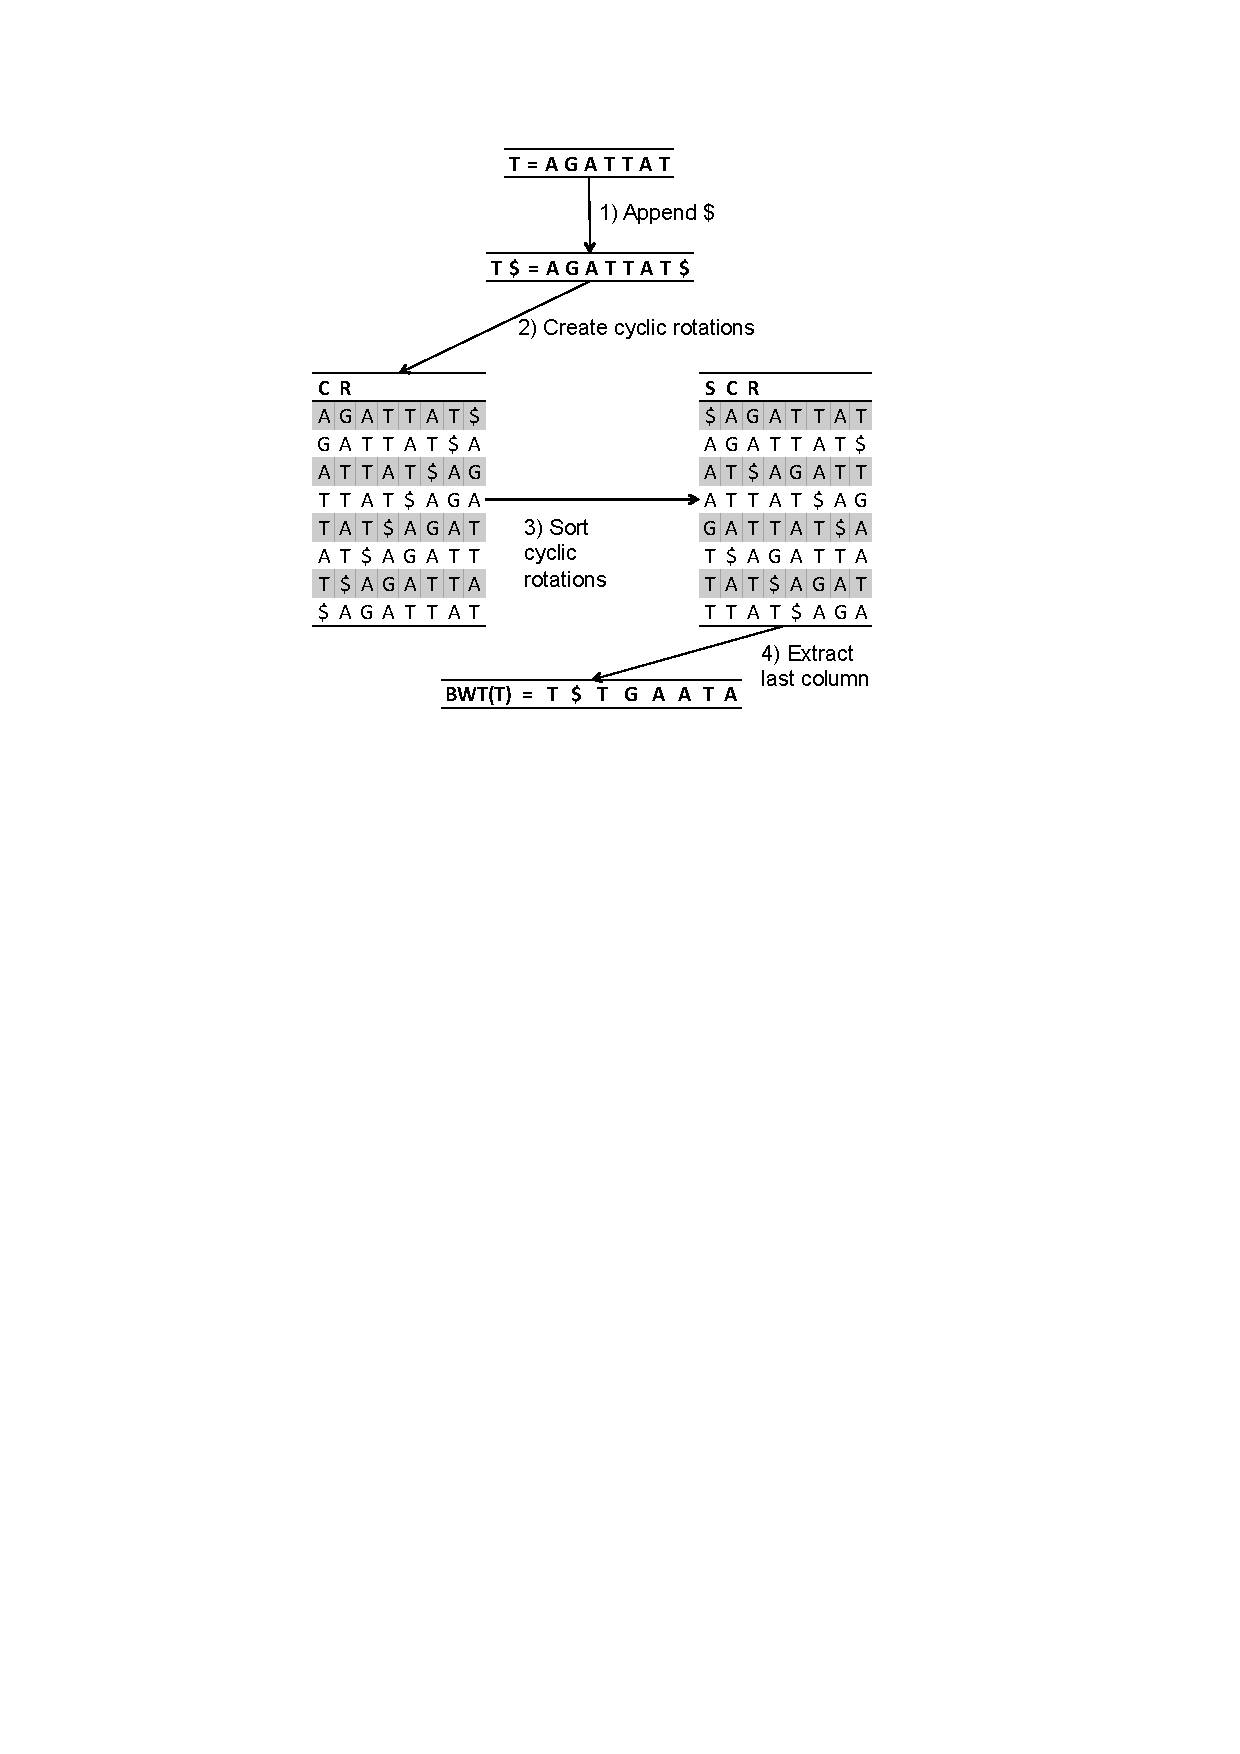
\includegraphics{fig/bwt.pdf}
\caption{Primjer algoritma BWT transormacije niza \textit{T = AGATTAT}}
\label{fig:bwt}
\end{figure}

Bitno je primjetiti kako je BWT transformacija niza srodna sufiksnoj listi \textit{SA} \engl{suffix array}. Sufiksna lista
je struktura podataka koja se često koristi u algoritmima nad tekstom. Njenu formulaciju
nećemo detaljno objašnjavati, materijali na temu su široko dostupni. Sličnost između BWT
transformacije i \textit{SCR} tablice korištene u BWT transformaciji ilustrirana je slikom \ref{fig:bwt_sa}.

\begin{figure}[!htb]
\centering
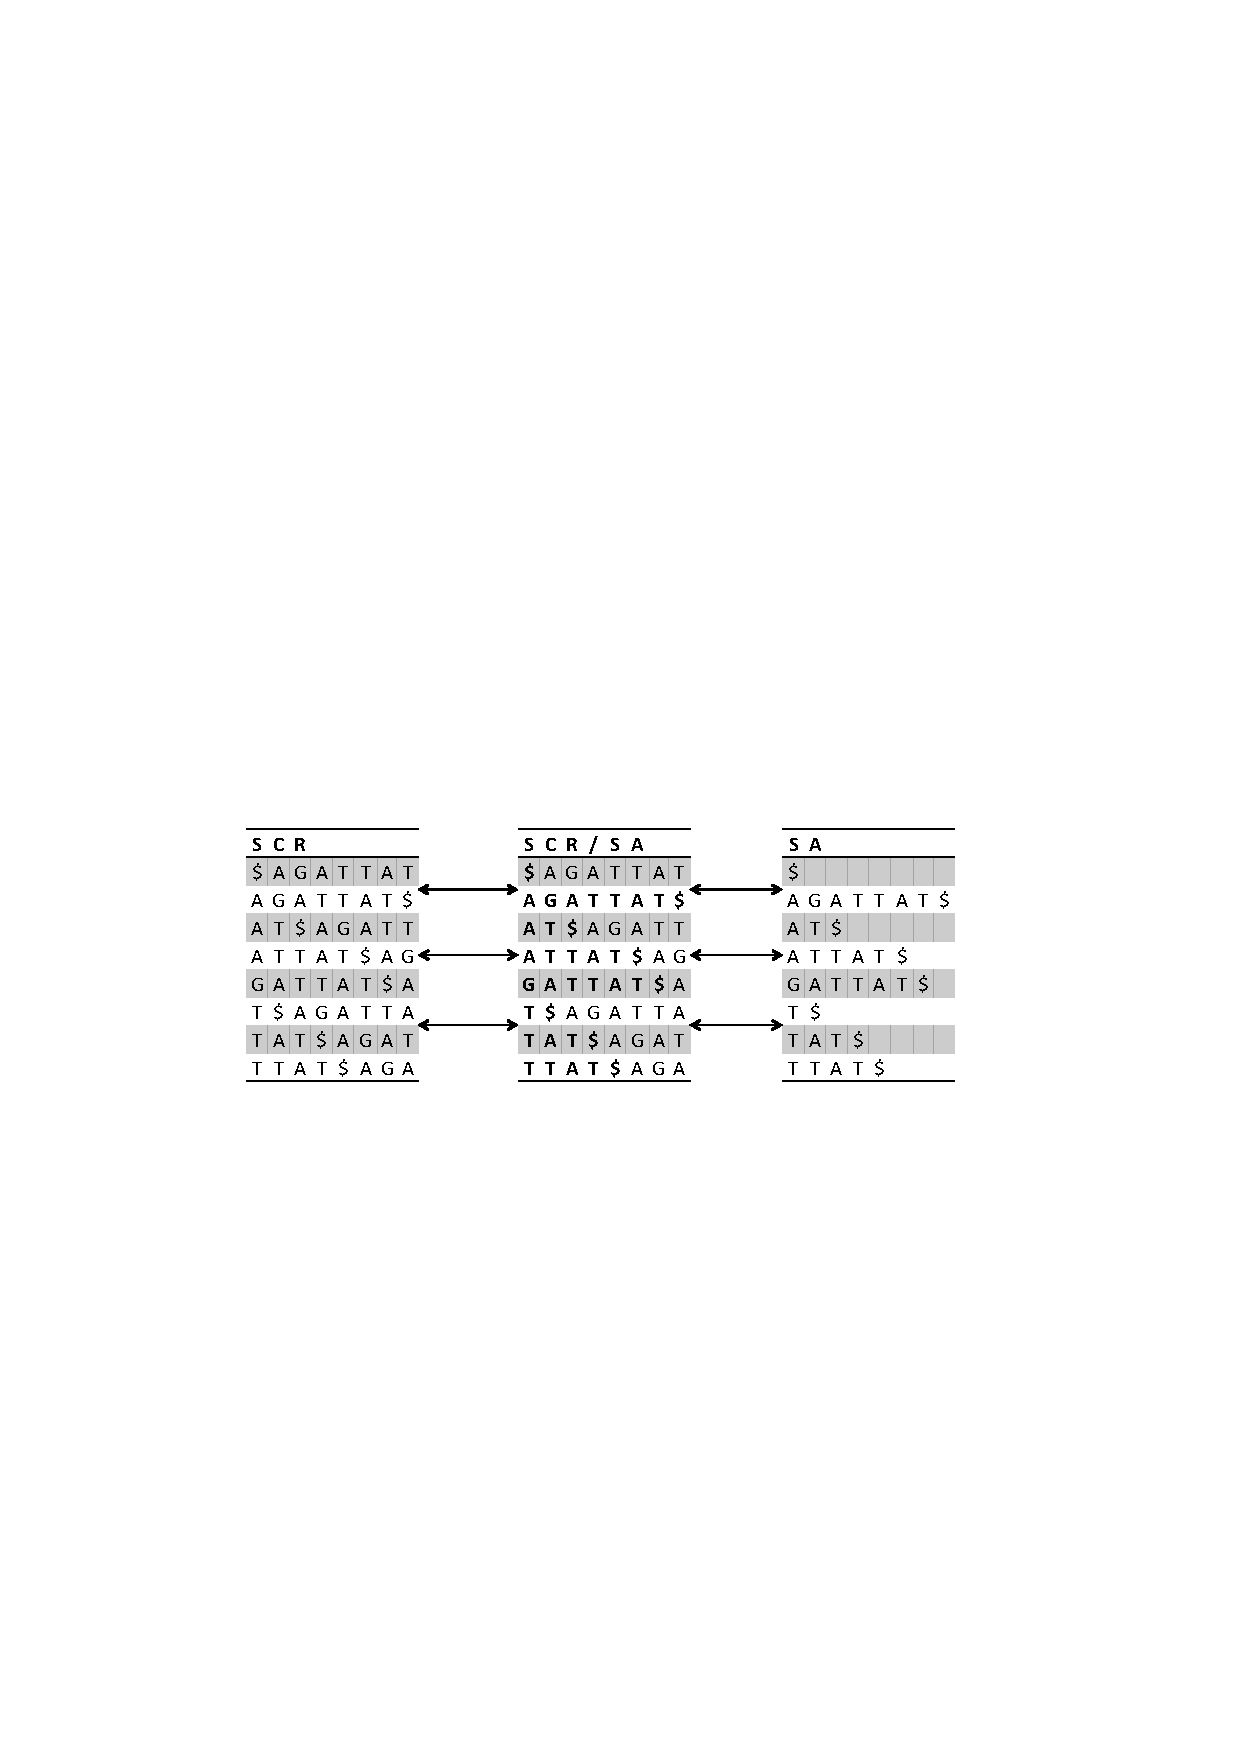
\includegraphics{fig/bwt_sa.pdf}
\caption{SCR tablica BWT tranfsformacije i sufiksna lista za niz \textit{T = AGATTAT}}
\label{fig:bwt_sa}
\end{figure}

\subsection{LF-mapiranje}

LF-mapiranje \engl{last-to-first mapping} opisuje relaciju između posljednjeg
stupca \textit{SCR} tablice (označenog \textit{L}) i prvog stupca te iste tablice (označenog
\textit{F})\footnote{Primjetimo da je \textit{L} isti stupac
koji definira BWT transformaciju.}. LF-mapiranje postulira da
\textit{i}-to pojavljivanje znaka \textit{c} unutar stupca \textit{L} korespondira
\textit{i}-tom pojavljivanju tog istog znaka unutar stupca \textit{F}. Pri tome "korespondira"
znači da se radi o istom znaku unutar originalnog niza \textit{T}. Jednostavan dokaz ovog
iskaza moguće je naći u \cite{singer_2012}.

Brza implementacija LF-mapiranja (konstantne
vremenske složenosti) može se ostvariti implementacijom dviju pomoćnih tablica. Tablica
prefiksnih suma \textit{C} \engl{prefix-sum table} niza \textit{T} za svaki znak \textit{c}
pohranjuje broj znakova u \textit{T} koji su manji od \textit{c}. Tablica pojavljivanja
\textit{Occ} \engl{occurrence table} pohranjuje informaciju koliko puta se neki znak
\textit{c} pojavio u nizu \textit{T} do pozicije \textit{i} (isključujući znak točno na
poziciji \textit{i}). Korištenjem tablica \textit{C} i \textit{Occ} LF mapiranje za
\textit{T\textsuperscript{BWT}} (koji odgovara stupcu \textit{L}) računa se na sljedeći način,
za znak \textit{c} na poziciji \textit{i}:

\begin{enumerate}
  \item{Pronađi broj pojavljivanja \textit{c} u \textit{T\textsuperscript{BWT}} do pozicije \textit{i} unutar tablice \textit{Occ}}
  \item{Pronađi broj znakova manjih od \textit{c} u \textit{T\textsuperscript{BWT}} unutar tablice \textit{C}}
  \item{Zbroj pronađenih vrijednosti je indeks korespondirajućeg znaka u stupcu \textit{L}}
\end{enumerate}

\subsection{Rekonstrukcija originala}

Na temelju transformiranog niza \textit{T\textsuperscript{BWT}} moguće je rekonstruirati
originalni niz \textit{T} korištenjem LF-transformacije. Postupak je jednostavan, ako imamo
na umu definiciju LF-transformacije i činjenicu da je prvi znak u \textit{T\textsuperscript{BWT}}
zasigurno posljednji znak niza \textit{T} (ovo proizlazi iz činjenice da smo pri postupku BWT
transormacije na početak niza umetnuli znak '\$').

Rekonstrukcija niza \textit{T} obavlja se unatrag, od posljednjeg znaka prema prvom. Postupak
je sljedeći:

\begin{enumerate}
  \item{Prvi znak iz \textit{T\textsuperscript{BWT}} je posljednji znak iz \textit{T}, zabilježimo ga}
  \item{LF-transformacijom pronađimo \textit{F}-indeks  posljednjeg zabilježenog znaka \footnote{
    U ovom trenutku nemamo tablicu \textit{SCR}, zanima nas samo indeks}}
  \item{Dobiveni \textit{F}-indeks u \textit{T\textsuperscript{BWT}} nizu ukazuje na znak koji u nizu
    \textit{T} prethodi posljednjem zabilježenom znaku (posljedica rotacije pri konstrukciji \textit{SCR})}
  \item{Zabilježimo znak na \textit{F}-indeks poziciji niza \textit{T\textsuperscript{BWT}} u rekonstrukciju}
  \item{Ako posljednji zabilježeni znak nije '\$', vraćamo se na korak 2.}
\end{enumerate}

Opisani postupak vizualiziran je na slici \ref{fig:lf_reconstruct}. Bitno je primjetiti kako pri
rekonstrukciji originala nismo koristili ništa osim transformiranog niza \textit{T\textsuperscript{BWT}}
i LF-mapiranja (koje se ostvaruje tablicama \textit{C} i \textit{Occ}).

\begin{figure}[!htb]
\centering
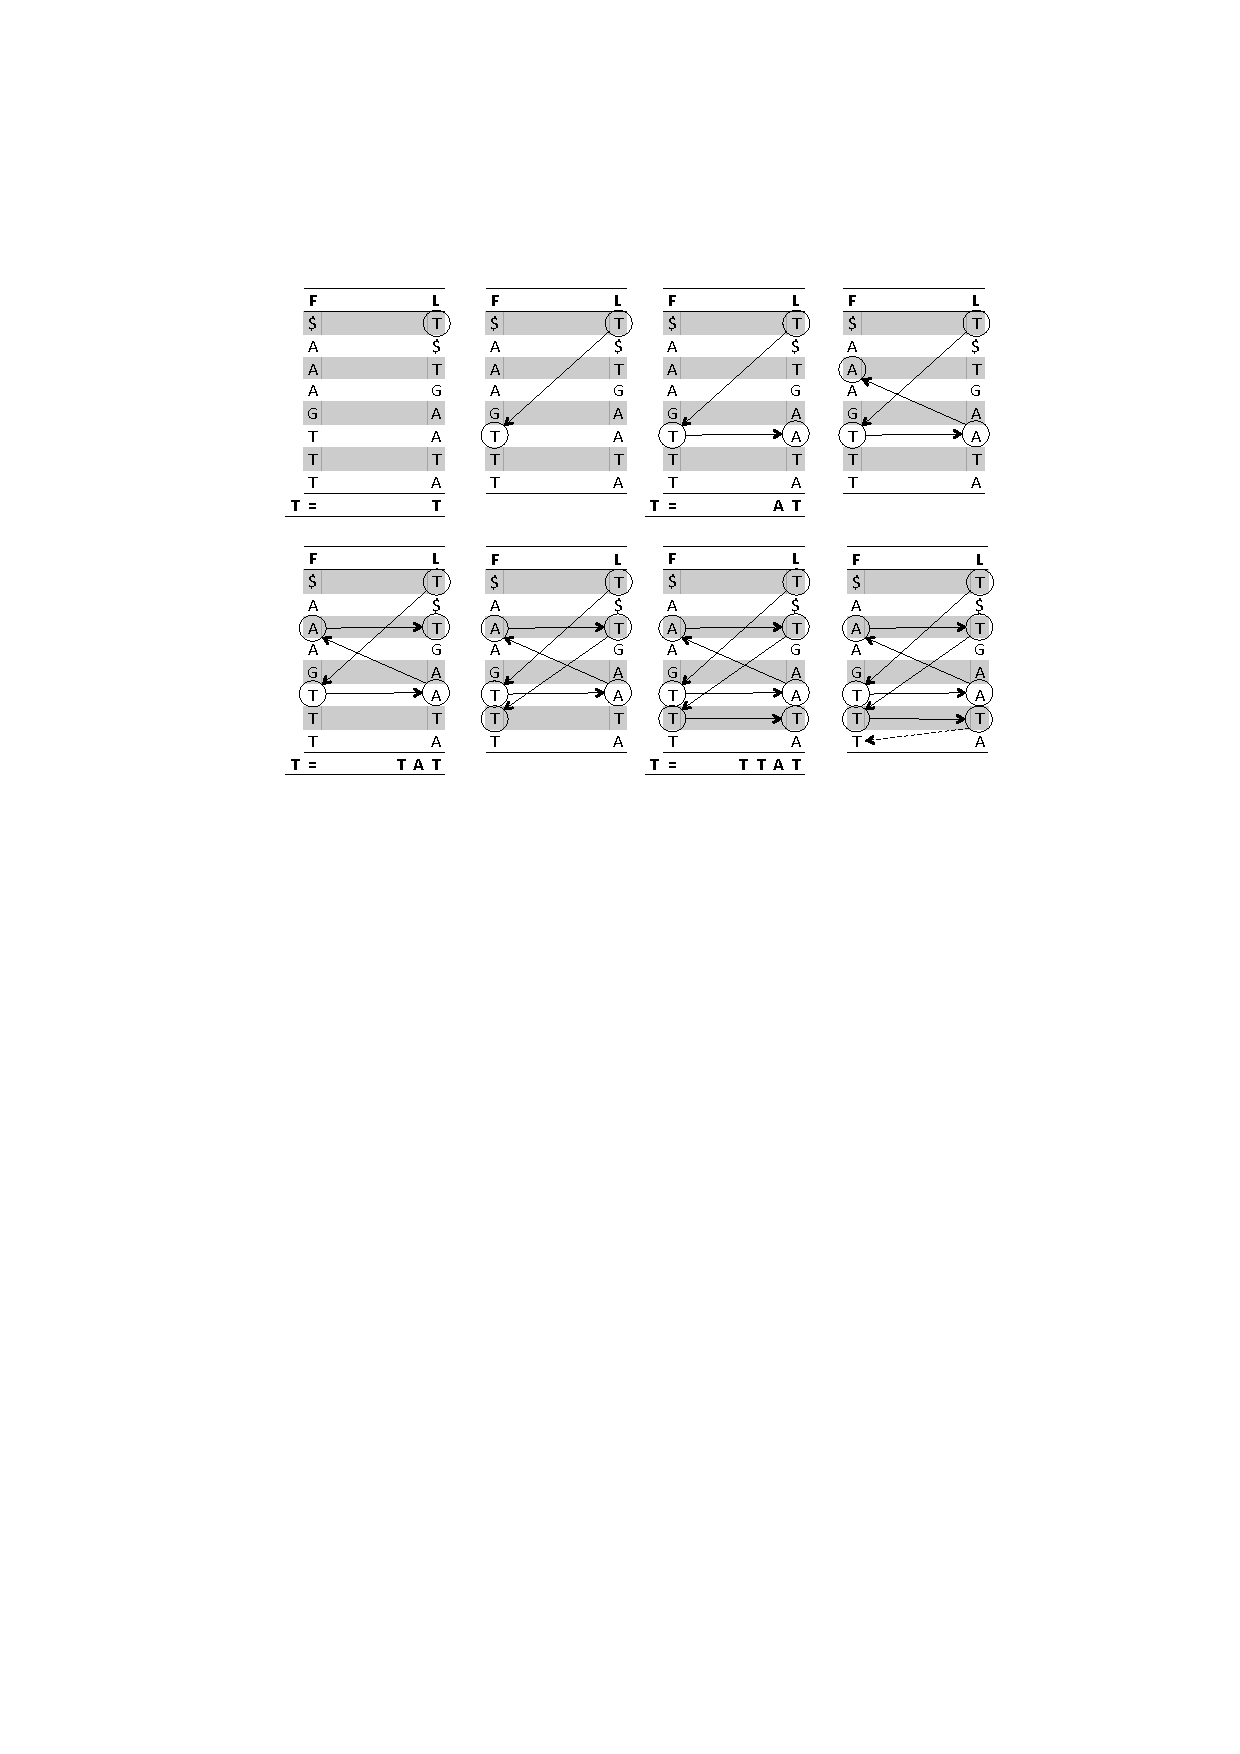
\includegraphics{fig/lf_reconstruct.pdf}
\caption{Primjer rekonstrukcije originala iz transformiranog niza \textit{T\textsuperscript{BWT}}}
\label{fig:lf_reconstruct}
\end{figure}

\subsection{Pretraživanje}
\label{sec:pretrazivanje}

Transformirani niz \textit{T\textsuperscript{BWT}} može se koristiti i za pretraživanje
originalnog teksta \textit{T}. Algoritam pretraživanja vrlo je sličan rekonstrukciji
originala. Bazira se zapravo na poznatom načinu pretraživanja sufiksnih polja, kao
što je već spomenuto, BWT transformacija i sufiksno polje nekog niza su skoro ekvivalentni.

Algoritam pretraživanja pojavljivanja niza \textit{Q} unutar niza \textit{T} na temelju
BWT transforacije \textit{T\textsuperscript{BWT}} bazira se na sljedećim konceptima:

\begin{itemize}
  \item{Pretraživanje se vrši po znakovima \textit{Q} unatrag (od zadnjeg prema prvom)}
  \item{Prate se početni i krajnji indeks sufiksa (\textit{SCR} tablice) unutar kojih su moguće podudarnosti}
  \item{U svakom koraju (procesiranom znaku iz \textit{P}) se područje mogućih podudarnosti smanjuje}
\end{itemize}

Ako početni indeks označimo \textit{ps} \engl{pointer start}, a krajnji indeks \textit{pe}
\engl{pointer end}, tada se algoritam izvršava sljedećim koracima:

\begin{enumerate}
  \item{Inicijaliziraj indekse \textit{ps} i \textit{pe} tako da obuhvaćaju cijelu tablicu \textit{SCR}}
  \item{Odaberi prvi neobrađeni znak \textit{c} iz niza \textit{Q}, počevši od kraja}
  \item{Unutar područja među indeksima nađi prvo i posljednje pojavljivanje znaka \textit{c}
    \footnote{Učinkovita implementacija pretraživanja ne izvršava ovaj korak, navodimo ga
    samo radi opisa rada algoritma.}}
  \item{Izračunaj \textit{L}-indekse nađenih pojavljivanja koristeći LF-mapiranje}
  \item{Ako postoje neobrađeni znakovi u \textit{Q}, vrati se na korak 2.}
\end{enumerate}

Navedeni koraci algoritma formulirani su kako bi bili što jasniji. Opis prikladniji
za izravnu računalnu implementaciju može se naći u radu \cite{singer_2012}. Slika
\ref{fig:sa_search} prikazuje korake pretraživanja za \textit{Q = TAT}.

\begin{figure}[!htb]
\centering
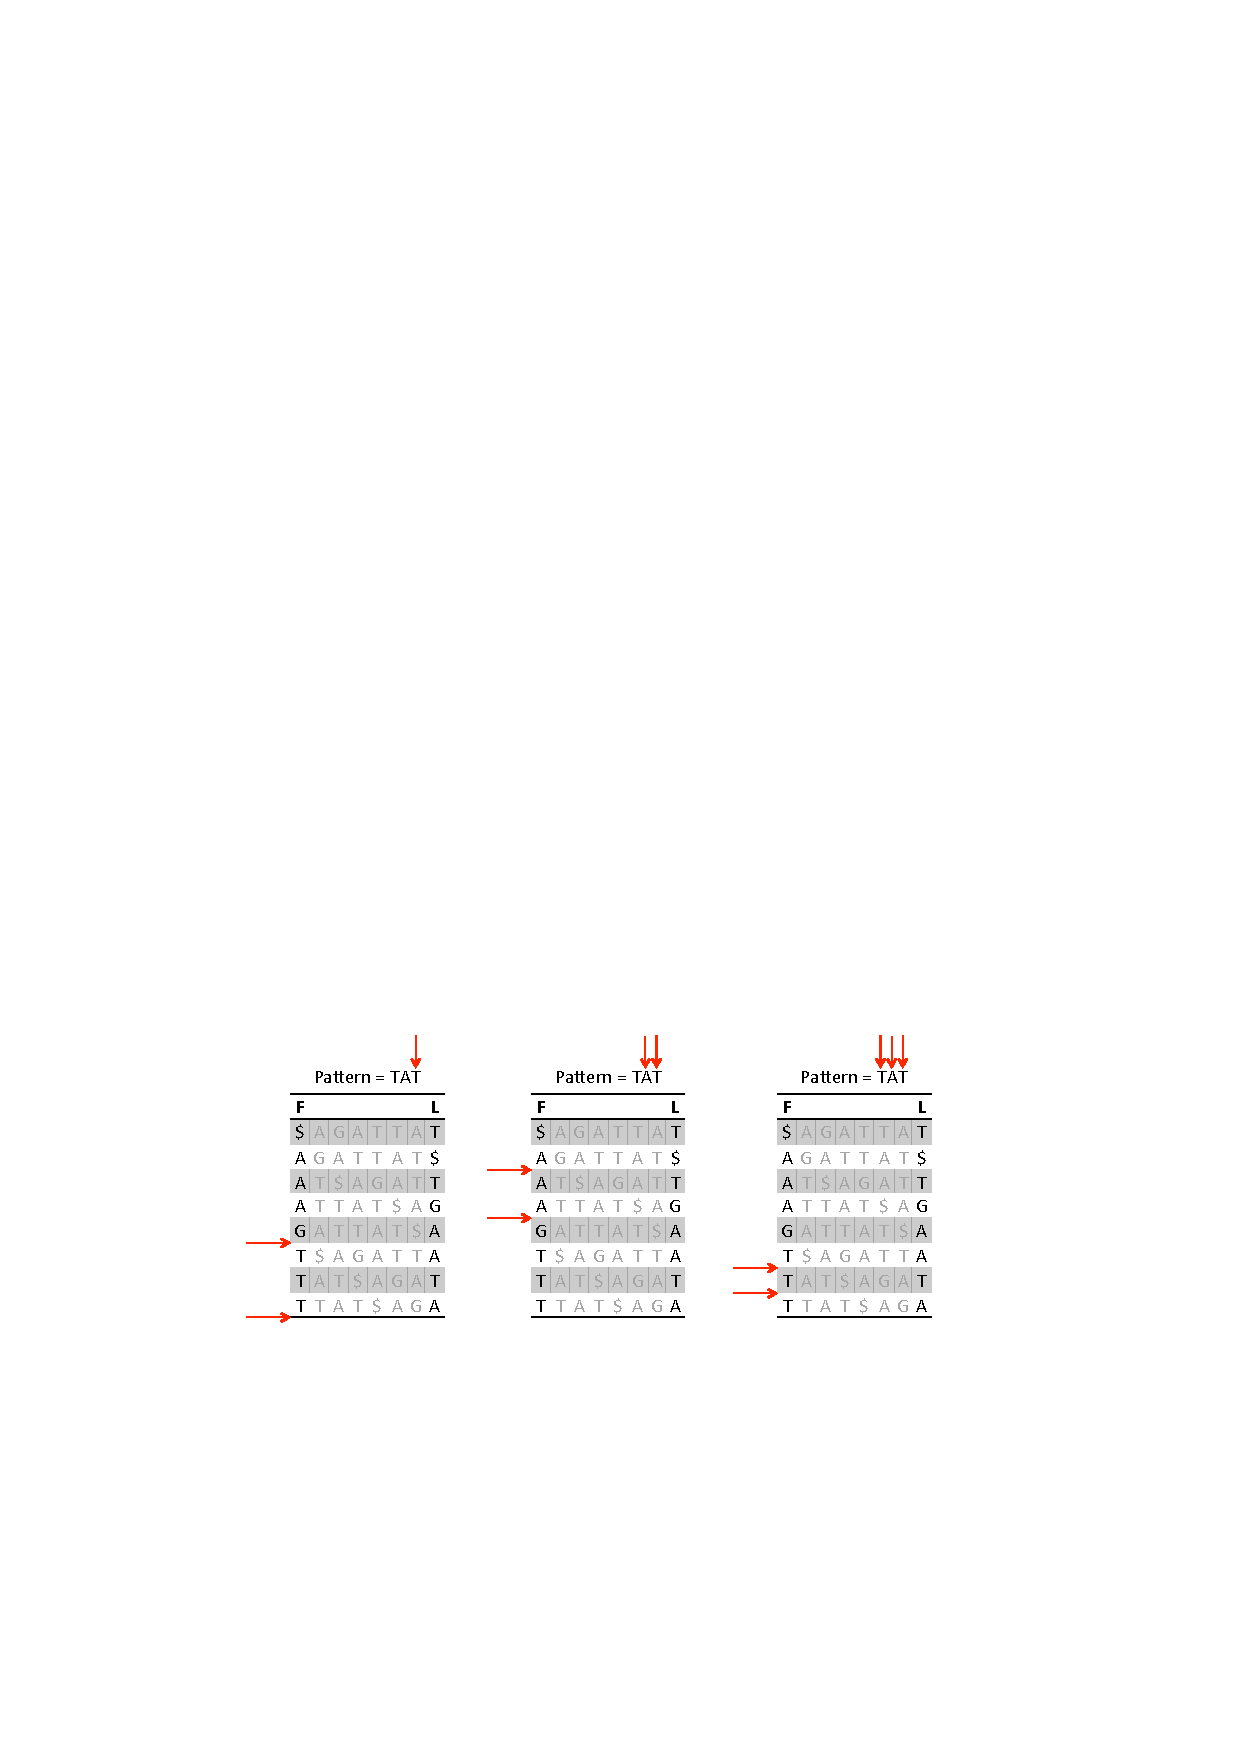
\includegraphics{fig/sa_search.pdf}
\caption{Primjer pretraživanja teksta korištenjem transformiranog niza \textit{T\textsuperscript{BWT}}}
\label{fig:sa_search}
\end{figure}

\section{Analiza složenosti algoritma}

Glavni razlog za razvoj FM-indeksa je povećanje efikasnosti pretraživanja dugih nizova
(poput genotipa). U ovom poglavlju će se razmotriti složenost pretraživanja korištenjem
FM-indeksa, sa teoretskog stanovišta. Pri tome nas zanima složenost korištenja
izgrađenog indeksa za neki niz, a ne složenost stvaranja indeksa.

\subsection{Vremenska složenost}

Razmotrimo vrijeme pronalaska pojavljivanja niza \textit{Q} unutar niza \textit{T}, na
način opisan u poglavlju \ref{sec:pretrazivanje}. Iz algoritma je vidljivo da je
potreban jedan korak za svaki znak u \textit{Q}, dakle pretraživanje ima linearnu
složenost s obzirom na duljinu \textit{Q}. Svaki od tih koraka svodi se na dvije
operacije LF-mapiranja, koje ima konstantnu vremensku složenost (ne ovisi o duljinama
nizova \textit{T} i \textit{Q}).

Važna napomena je da prolazak kroz znakove niza \textit{Q} može biti prekinut u slučaju
da se utvrdi da nema pojavljivanja \textit{Q} unutar \textit{T}, što se može desiti
u bilo kojem trenutku prolaska kroz \textit{Q}.

Dakle, vremenska složenost pretraživanja je generalno linearna s obzirom na duljinu
niza \textit{Q}.

\subsection{Memorijska složenost}

Memorijska (prostorna složenost) je razmatranje utroška memorije na potporne
strukture podataka FM-indeksa. Podatci koji se koriste su transformirani niz
\textit{T\textsuperscript{BWT}} (odnosno sufiksno polje) te tablice \textit{C}
i \textit{Occ} korištene za LF-mapiranje.

Sufiksno polje ima jednak broj elemenata kao i originalni niz \textit{T}. U
tom smislu je memorijska složenost polja linearna s obzirom na duljinu \textit{T}.
Isto vrijedi i za transformirani niz \textit{T\textsuperscript{BWT}}. Prostorni
utrošak sufiksnog polja može se smanjiti na više načina, a niz \textit{T\textsuperscript{BWT}}
je često oblika pogodnog za komprimiranje, ali obje tehnike izlaze izvan okvira
ovog rada.

Tablica prefiksnih suma \textit{C} pohranjuje po jedan cijeli broj za svaki
element abecede niza \textit{T}. Iako je u teoriji taj broj ograničen samo
duljinom niza \textit{T}, u praksi je zapravo vrlo malen te tablica \textit{C}
ne predstavlja problem u kontekstu zauzeća memorije.

Tablica pojavljivanja \textit{Occ} (u naivnoj implementaciji) pohranjuje po
jedan cijeli broj za svaku poziciju niza \textit{T}, za svaki element abecede \textit{T}.
Primjećujemo linearnu složenost s obzirom na duljinu niza \textit{T}. S obzirom
na potencijalno ogromne duljine nizova koje želimo moći pretraživati, ovo je problem.
Postoji više pristupa "kodiranja" tablice \textit{Occ}. Unutar ovog rada, zadatak
je implementirati FM-indeks korištenjem stabla valića.


\chapter{Stablo valića}

\chapter{Implementacija i testiranje}

\chapter{Zaključak}
Zaključak.

\bibliography{literatura}
\bibliographystyle{unsrt}

\chapter{Sažetak}
Sažetak.

\end{document}
